\clearpage

\chapter{Weitere Diagramme}

\section{Zustandsdiagramm - Memorykarte}

\begin{figure}[!h]
	\centering
    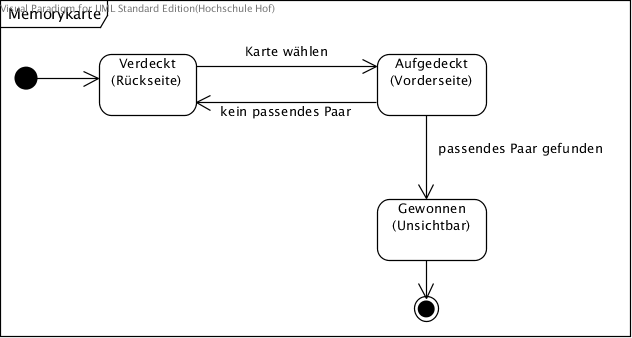
\includegraphics[width=\textwidth]{./ZD_Memorykarte.png}
	\label{layout_gesamt}
\end{figure}
\subsection{Beschreibung}
Die Karte kann die drei Zustände Verdeckt, Aufgedeckt und Gewonnen annehmen. Wird eine verdeckte Karte ausgewählt, wechselt sie in den Zustand Aufgedeckt. Der Zustand Aufgedeckt kann entweder durch die Feststellung, dass ein passendes Kartenpaar gefunden wurde in den Zustand Gewonnen übergehen, oder falls es sich um nicht zwei übereinstimmende Karten handeln, wieder in den Zustand Verdeckt wechseln.


\clearpage
\section{Aktivitätsdiagramm - Spielablauf}

\begin{figure}[!h]
	\centering
    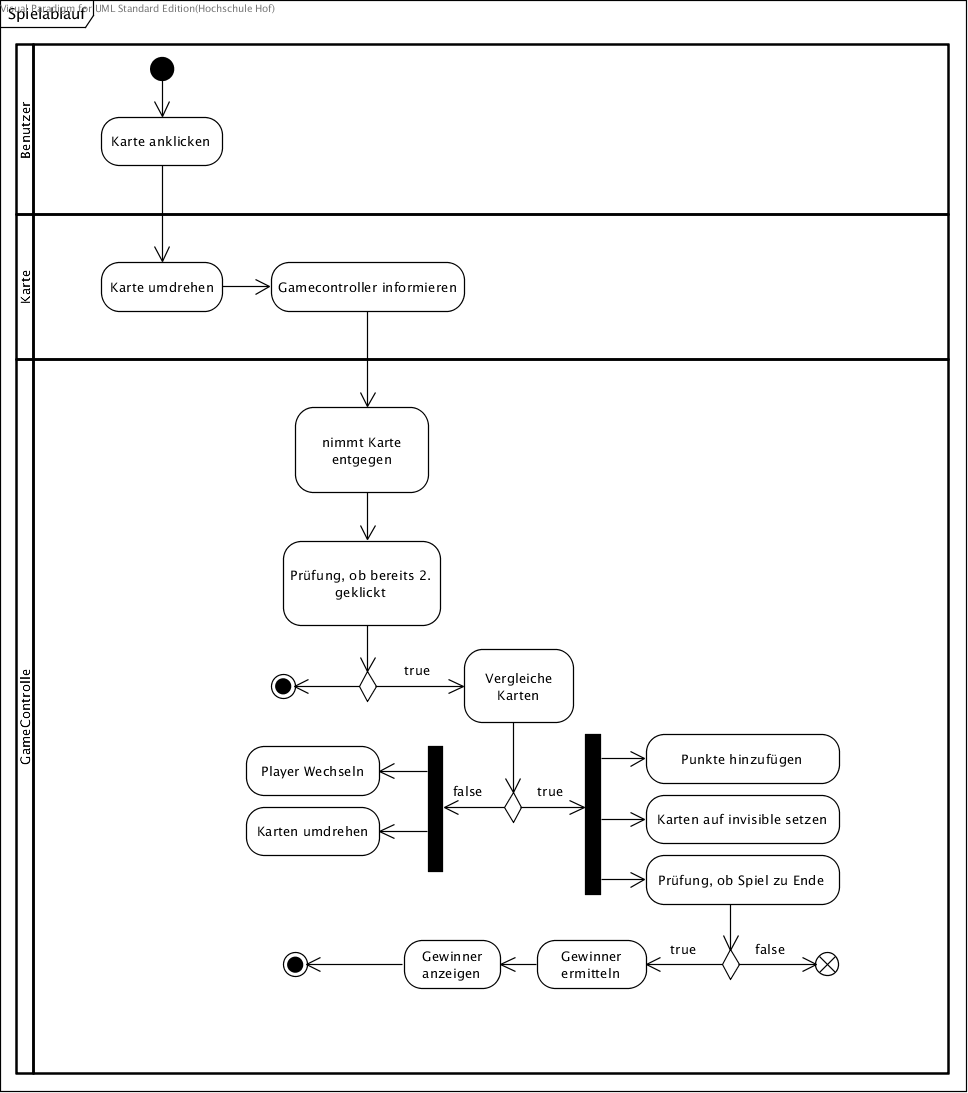
\includegraphics[width=\textwidth]{./AD_Spielablauf.png}
	\label{layout_gesamt}
\end{figure}
\subsection{Beschreibung}
Der Spielablauf beginnt mit dem Klick auf eine Karte durch den Benutzer. In der Klasse Card (Karte) wird die Funktion zum Umdrehen der Karte aufgerufen und der GameController wird informiert, dass eine Karte ausgewählt wurde. Der GameController nimmt die Information über die Karte entgegen und prüft, ob es sich um die 2. ausgewählte Karte handelt. Ergibt diese Prüfung false, ist die Aktivität beendet. Erst durch den nächsten Klick auf eine Karte, wird die Aktivität wiederholt. Hat die Prüfung true ergeben, erfolgt ein Vergleich der durch den Benutzer gewählten Karten. False führt dazu, dass der Spieler gewechselt wird, die Karten wieder umgedreht werden und die Aktivität beendet ist. Bei True werden dem aktuellen Spieler Punkte hinzugefügt, die Karten auf invisible gesetzt und eine Prüfung angestoßen, ob das Spielende erreicht ist. Ist das Spielende nicht erreicht, endet die Aktivität. Ergibt die Prüfung, dass das Spielende erreicht ist, wird der Gewinner ermittelt und angezeigt. Hier endet die Aktivität.


\clearpage
\section{Komponentendiagramm}

\begin{figure}[!h]
	\centering
    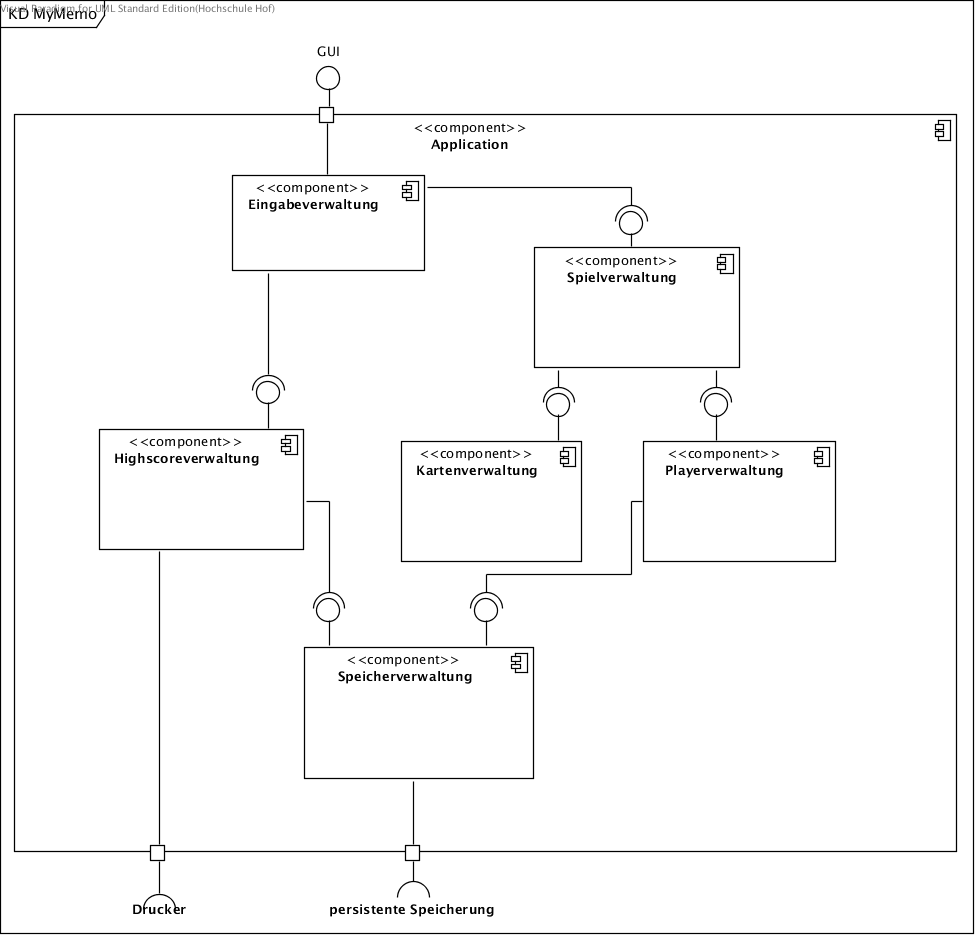
\includegraphics[width=\textwidth]{./komponentendiagramm.png}
	\label{layout_gesamt}
\end{figure}
\subsection{Beschreibung}
Um eine bessere Übersicht zu erhalten, wurden die Klassen aus dem Klassendiagramm zu Komponenten zusammengefasst.\\

\noindent \textbf{Eingabeverwaltung: }Menue, InputData\\
\textbf{Spielverwaltung: }GameField, GameLayout, GameController\\
\textbf{Playerverwaltung: }Player, Playerpool\\
\textbf{Kartenverwaltung: }Card\\
\textbf{Highscoreverwaltung: }Highscore, HighscoreData\\
\textbf{Speicherverwaltung: }SaveObject, HddSave\\

Das Komponentendiagramm stellt dar, wie die einzelnen Komponenten des Systems aufeinander zugreifen.\\
Die Applikation selbst hat Schnittstellen zur Technischen Schicht in Form von Drucker und persistenter Speicherung. Eine weitere Schnittstelle besteht zur Präsentationsschicht, im Diagramm zusammengefasst unter GUI.



\clearpage
\section{Paketdiagramm}

\begin{figure}[!h]
	\centering
    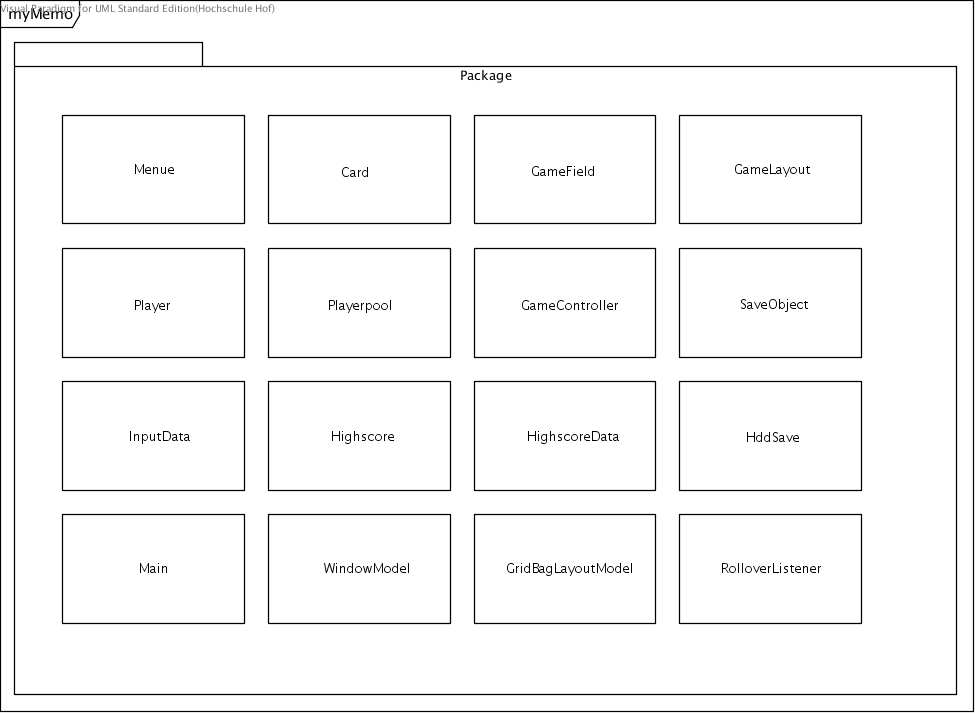
\includegraphics[width=\textwidth]{./paketdiagramm.png}
	\label{layout_gesamt}
\end{figure}
\subsection{Beschreibung}
Da das System ohne die Verwendung verschiedener Packages geplant und umgesetzt wurde, erfolgt die Darstellung des Paketdiagramms in obiger Form.


\clearpage
\section{Verteilungsdiagramm}

\begin{figure}[!h]
	\centering
    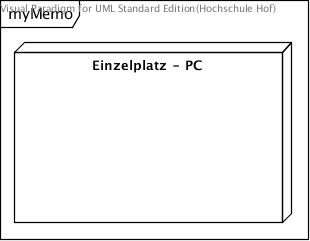
\includegraphics[width=\textwidth]{./verteilungsdiagramm.png}
	\label{layout_gesamt}
\end{figure}
\subsection{Beschreibung}
Die Software kommt ausschließlich auf Einzelplatz-PCs zum Einsatz. Es erfolgt keine Verteilung auf verschiedene Systeme. Deshalb enthält das Verteilungsdiagramm ausschließlich den Einzelplatz-PC.




